\chapter{Simulations}
\label{ch:simulations}

\section{Why simulations?}

Simulations are used to check if the data we see is what we expected.



\section{Monte Carlo extensive air shower simulation}

For the simulation of air showers there are several programs available;
\corsika, AIRES, and ... \corsika was chosen because it is still being
actively worked on, unlike AIRES which received its last update in 2006.
\corsika also includes updated models based on recent LHC data.
Moreover, \corsika is also used by most other cosmic-ray experiments.
\corsika v74000 is used, which includes models updated based on LHC data.

\corsika provides the choice from many models for various interactions.
For high energy hadronic interactions; DPMJET 2.55, EPOS LHC, NEXUS
3.97, QGSJET 01C (enlarged commons), QGSJETII-04
[http://inspirehep.net/record/1242711/files/epjconf_isvh2012_02001.pdf],
SIBYLL 2.1, and VENUS 4.12 are available. For hadrons with energies
below \SI{80}{\giga\electronvolt} GHEISHA 2002d (double precision),
FLUKA, or URQMD 1.3cr can be selected. Electromagnetic interactions can
be treated by EGS4 [http://rcwww.kek.jp/research/egs/] code or by NKG
formulas.

QGSJETII, GHEISHA and EGS4 were chosen. One configuration of \corsika
was compiled and all showers were run using that executable.

The simulations are steered by an input file, many parameters can be set
here. The default options were used whenever applicable and trusting in
sensibly chosen defaults. The seeds for the random number generators
(first for the hadron shower, second for EGS4) are different for each
run. The seed values are (by us) also used as identifiers for the
simulations, so each combination of two seeds is unique in dataset of
simulations. Only one shower is simulated per run. Each run is for a
specific particle with a specified energy between
\SIrange{$10^{12}$,$10^{18}$}{\electronvolt} in steps of $\log E = .5$.
The zenith angle is also set for each run and can be varied from
\SIrange{0,60}{\degree} in steps of \SI{7.5}{\degree}. The azimuthal
angle is usually set to \SI{0}{\degree} (\hisparc coordinate system). 
The magnetic field values have been modified to values for Amsterdam [ref].

Energy cuts \SI{300}{\mega\electronvolt} for hadrons and muons, and
\SI{3}{\mega\electronvolt} for electrons and photons. Below these
energies the particles are quickly stopped/slowed by the atmosphere
decay [ref PDG]. The observation level for all runs is set to
\SI{10}{\meter} above sea level, which is relevant for the Science Park
where ground level is \SI{3.7}{\meter} below sea level, and the detector
are on the roofs of buildings.


\subsection{Simulations catalogue}

Using Stoomboot a collection of over \num{70000} simulated showers has
been created. This data is stored on the \hisparc data server (trave)
which has \SI{37}{\tera\byte} space. This space is shared with the raw
\hisparc data, \knmi lightning data, and some analysis files from
various \hisparc collaborators.

For easy use with the \sapphire framework the \corsika simulations are
converted from the binary/fortran data format to \hdf format. This is
done using a modified version of the the Python \corsika Reader by J.
Gonzalez from Auger. After the initial conversion further optimisation
is performed by sorting and indexing the 'x' coordinate column for the
particles. In the detector simulation particles are queried from the
\corsika data file using x and y coordinates. With the index it is very
easy for the software to know which part of the data it needs, since the
data is sorted (on disk) only a small part of the data needs to be read
into memory, if the data was not sorted more chunks of the file would
need to be read into memory. In some cases the sorting speeds up
simulations by a factor of 50.

Given the high abundance of protons as primary particles and iron with a
relative high abundance for heavier nuclei we have mostly focused on
those two particles for the simulations. However, some other primaries
have also been used. For protons (and iron??) all possible combinations
of energy and zenith have been simulated at least x times. More showers
are available at lower zenith angles and around
\SI{$10^{15}$}{\electronvolt}. Larger showers take up much more disk
space and time to compute. In \ref{fig:simulations_proton_energy_zenith}
the number of simulations for each combination of parameters can be seen.
(at time of writing..)

\todo{Update plot with intermediate energies, and 'color bar'}

\begin{figure}
    \centering
    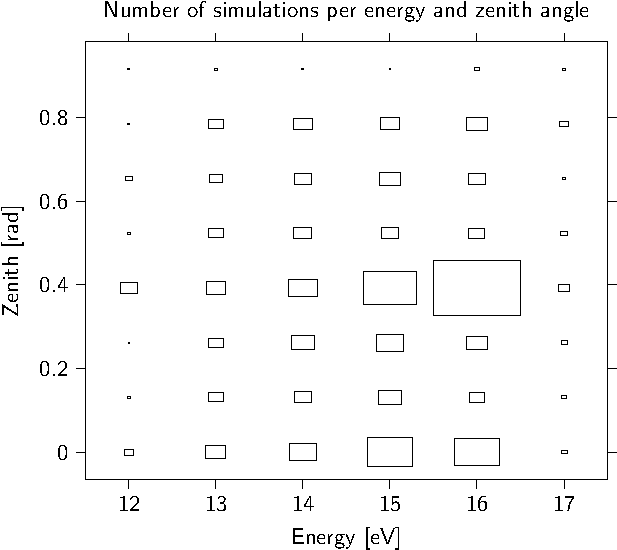
\includegraphics[width=0.7\linewidth]
        {plots/simulations/proton_energy_zenith}
    \caption{\captitle{Proton simulations overview.} The area of the
             rectangles indicate the number simulations with that energy
             and zenith combinations.}
    \label{fig:simulations_proton_energy_zenith}
\end{figure}


\section{Detector simulation}

trigger efficiency
simulations
every step eplained and understood
trigger representateren

Simulations for various starting parameters were run. The combinations
of two seeds that can be given in the input where chosen to be unique
for each simulated shower, regardless of other parameters.


\subsection{Stoomboot}

To run a significant number of simulations the local Nikhef
computer cluster 'Stoomboot' was utilized. This cluster used to have
around 300 CPUs available, but was expanded in February 2014 to 850
CPUs. Job queueing uses a fair-use policy to give each group at Nikhef
equal access to computation time.

Simulation time for each simulation is different because the number of
particles in a simulations will be different each run. Stoomboot has a
maximum job time of \SI{96}{\hour}. This allows for showers with primary
energies upto \SI{10e17}{\electronvolt}, which take around 60 hours to
complete. Lower energy showers take far less time (energy proportional
to time?), so a large sample of showers can easily be generated by
running many jobs simultaneously.

Since there are also showers of energies \SI{10e17}{\electronvolt} we
want to have some simulations at higher energies. So during the
Christmas holidays we ran 200 jobs at energies upto
\SI{10e18}{\electronvolt}. These jobs sometimes took over
\SI{400}{\hour} to complete. This was a special run where the maximum
jobs times had to be explicitly set by the administrators. In total we
used \SI{50}{\year} of compute time to generate the simulation sample.

\todo{Determine compute time used on Stoomboot}


\section{Simulations on clusters}

We have some simple simulations for flat and curved shower fronts.
Does not include particle density.
Detector/trigger/response simulations. Do we understand what we see?


\section{Realistic simulation}

\todo{Simulation with fluxes and azimuth/zenith distributions.}

\todo{Acceptance; angle, energy and particles.}

See detector response, cluster response and calibration.


\section{Analysis}

\todo{Information about shower from simulations}

Timing information, front shape, timing distribution, particle arrival times..
Air pressure dependence.

Particle density, effect of inclination..
